\documentclass[output=paper]{langscibook}
\ChapterDOI{10.5281/zenodo.5578844}

\author{Doreen Enyonam Esi Yegblemenawo\affiliation{Department of French Education, University of Education, Winneba, Ghana} and Stella Afi Makafui Yegblemenawo\affiliation{Department of Language and Communication Sciences, Kwame Nkrumah University of Science and Technology, Kumasi, Ghana}}

\title[Documenting praise names \textit{ahanoŋkɔ} among Ewes]{Documenting praise names \textit{ahanoŋkɔ} among Ewes: A socio-semantic perspective}
\abstract{Names generally identify an individual and set him/her apart from other individuals. The Ewe (ISO639-3 [ewe])-speaking people of Ghana are known to have names which reflect an idea that a name giver or name bearer intends to put across. These names could be given due to, among others, circumstances under which the bearer was born, the day of birth, order of birth, or religious affiliations. Using a multifaceted approach in language documentation, this study focuses on a type of personal names termed {\textit{ahanoŋkɔ}} (which literally translates as ‘drinking name’ or ‘name used while drinking alcohol’) among the Ewe of southeast Ghana, and investigates the semantic perspective of these praise names; {\textit{ahanoŋkɔwo}}, as well as their social impact on the bearers and non-bearers of the names.}

% \Keywords{Praise names, Ewe, Ghana, Impact, Names, Semantics}
\begin{document}
\maketitle

\section{Introduction}
Names play a variety of roles in connecting a person to his or her identity and individuality. This means, each individual at birth, is given a personal name which is used to identify him or her. The Ewe people of Ghana are known to have names which reflect an idea that a name giver or bearer intends to put across. The names of the authors of this paper; {\textit{Enyonam}} and {\textit{Makafui}}, are examples of these personal names. The personal name \textit{Enyonam} is a short form of the actual name: {\textit{Nu sianu si Mawu wɔ nam la, enyo nam}}, meaning, ‘whatever God has done for me, it is well with me.’ It should be noted that, a name could be chosen later by the bearer or conferred on the bearer \citet{adjah2011name}.

The naming system among the Ewe people is not only rich and diverse, but also an interesting one, hence it is often an area of research. Quite a number of research works have been done on Ewe personal names, notable among these include \citet{Egblewogbe1977Ewe}, \citet{egblewogbe1984personal}, \citet{Atakpa1997}, \citet{adjah2011name} and \citet{abdul2014synchronic}. This research, however, concentrates on documenting praise names and their meanings among the Anlo-Ewe ethnic group of Ghana, using language documentation tools, while analysing the semantics and socio-cultural impacts on the bearers and non-bearers of these names. 
 
\subsection{The Ewe community in Ghana}
Ghana is made up of various ethnic groups which speak their own languages, with varied dialects, and have different cultural backgrounds. The Ewe ethnic group, which is largely resident in the area close to the eastern border of Ghana with Togo, is one of the numerous ethnic groups in Ghana.  The Ewe people speak Ewe (Éʋe or Éʋegbe) which is classified as a Kwa language. According to the Ethnologue report on Ghana, the number of speakers of the Ewe language is estimated to be about 3,320,000 \citep{Eberhard2020}. 

\begin{figure}
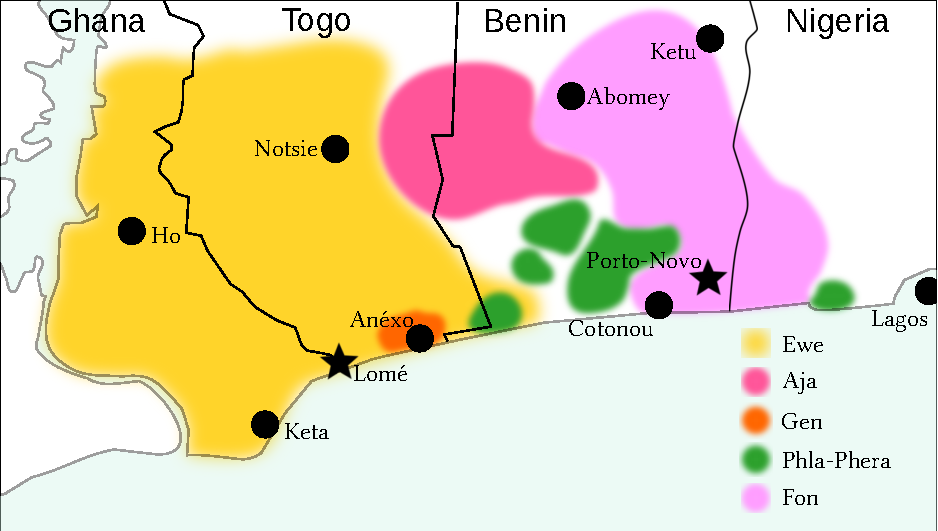
\includegraphics[width=.8\textwidth]{figures/gbe.pdf}
\caption{Geographical location of Ewe native speakers region (in yellow). CC-BY Mark Dingemanse and Sebastian Nordhoff.}
\end{figure}

In Ghana, there are several varieties of the Ewe language which include: \textit{Anlo (Aŋlɔ), Ʋedome, Tongu (Tɔŋu)}, etc. In this research, we are focusing on the Ewe dialect spoken by the Anlo people of Ghana.

\subsection{Typology of Ewe personal names}
Among the Ewe ethnic group of Ghana, one of the first rites of passage when a child is born is the `out-dooring' (\textit{viheheɖego}) and naming ceremony performed on the eighth day after birth. The name giver, usually the father of the child, or a designated paternal relative (that is, if the father died before the child’s birth), gives the child a name. The Ewe-speaking people of Ghana are well known to have names which reflect an idea that a name giver or name bearer intends to put across.
 
\citet{Egblewogbe1977Ewe} identifies ten naming systems among the Ewe people which he groups into four, namely: {\textit{dzɔdzɔmeŋkɔwo}} (natural names), {\textit{ŋkɔnanawo}}  (a given name at birth or taken later in life), {\textit{ŋkɔtsɔtsɔwo}} (names taken later in life or acquired names) and {\textit{subɔsubɔŋkɔwo}} (religious names). \citet{abdul2014synchronic} indicates that, the natural names which are inherent in a child, include birthday name ({\textit{azagbeŋkɔwo}}) given according to the day the child was born and circumstantial names where children are named based on circumstances surrounding their birth. The given names are conferred on a child at birth or sometimes taken up later in life. The acquired names are said to be taken on later in life. The religious names denote the religious affiliation of the child or his/her parents. \citet{agyekum2006sociolinguistic} in discussing Akan birthday names, termed it an automatic name every Akan child gets based on the day s/he was born even before s/he is officially named. This is the same for the Ewe child as he or she is also given day names depending on the day they were born as shown in \tabref{table:nonlin}.

\begin{table}
\caption{Ewe day names for male and female children \citep{Atakpa1997}\label{table:nonlin}}
\fittable{\begin{tabular}{llll}
\lsptoprule
Day (Eng.) & Day (Ewe) & Male child & Female child \\
\midrule
Sunday & Kɔsiɖa/Kwasiɖa & Kɔsie, Kwasi, Quarshie & Kɔshiwɔ, Awusi \\
Monday & Dzoɖa & Kɔdzo & Adzo, Adzowɔ\\
Tuesday & Braɖa/Blaɖa & Kɔbla, Kɔmla & Abla \\
Wednesday & Kuɖa & Kɔku & Aku, Akutɔ \\
Thursday & Yawoɖa & Yawo, Yao & Awo, Yawa, Yawɔ \\
Friday & Fiɖa & Kofi & Afi, Afiwɔ, Afitɔ \\
Saturday & Memleɖa/Memliɖa & Kɔmi & Ama, Ami, Ameyo \\
\lspbottomrule
\end{tabular}}
\end{table} 

Other naming categories include the circumstance of birth names such as {\textit{Adukpo}} [aɖukpó] ʻrubbish dumpʼ, {\textit {Modzinu}} [mɔ́dzínú] ʻsomething on the roadʼ, {\textit{Tsigbe}} [tsi gbe] ‘in the rainʼ. There are also ‘the mission of life’ (destiny) names such as {\textit{Kplɔla}} (leader/shepherd).

\subsection{Praise name {\textit{ahanoŋkɔ}} among Anlo-Ewe speakers}

Praise names describe in short cryptic forms the qualities and accomplishments of a status or a holder of the name \citep[216]{egblewogbe1984personal}. In Ewe, praise names are locally referred to as {\textit{ahanoŋ́kɔ́}} (pl. \textit{ahanoŋ́kɔ́wó}). This \citet{avorgbedor1983psycho} translates etymologically as `a drinking name'. The drink being  referred to, in this context, is an alcoholic drink, hence, it can be said to be an ‘alcohol-drinking-name’ or `a name used while drinking alcohol’. This name is sometimes called out when men gather to take alcoholic drinks in groups, but it does not mean it is mentioned out only within the context of drinking or taking alcohol.

Besides personal names given to an individual at birth, {\textit{ahanoŋkɔ}} is given to, or, taken up by the bearer himself later on in life as a result of peculiar characteristics or outstanding qualities which he exhibits.  Children, women, as well as men who were deemed unworthy, could not have an {\textit{ahanoŋkɔ}}.  Exceptions exist for a male child who exhibited extraordinary great qualities. He might earn an {\textit{ahanoŋkɔ}} but would have to wait till adulthood before having the name performed. {\textit{Ahanoŋkɔ}} could pass for a nickname but it is in reality, far more powerful than a mere nickname \citep{geurts2006enduring}

The Anlo-Ewe people are not the only ones who take up praise names. Other ethnic groups in Ghana such as Fantes and Ashantis equally take up praise names in their own unique forms. An example includes the form of praise appellations like \textit{Ahunabɔbirim} meaning `at whose sight you tremble' \citep{obeng2001african}. In a research on Bantu languages, \citet{finnegan2012oral} noted that praise names among the Bantu speakers were picked due to some striking quality of an object and were used for inanimate objects, birds, and animals, before they finally became names of people. As \citet{adjah2011name} rightly puts it, these praise names with appellations were acquired due to bravery or some other admirable quality and best describe the bearer of the name. Although most men take only one praise name, it is not out of place to find people responding to more than one {\textit{ahanoŋkɔ}}. It is common to find many people are known to have taken more than one {\textit{ahanoŋkɔ}} in order to increase the social and psychical dimensions of their ego \citep{avorgbedor1983psycho}.

\section{Why a praise name \textit{ahanoŋkɔ}?}

The reasons for taking up an {\textit{ahanoŋkɔ}} vary from person to person. It could be as a result of a heroic act performed by the bearer. These characteristics or qualities could be in the form of bravery, patience, resilience, or uniqueness. These praise names are called out loud or performed in order to cheer the bearers on. Each has a distinctive meaning and an interesting history behind it, which reflects not only the socio-cultural beliefs of the people, but also reveals the character traits of the bearer of the {\textit{ahanoŋkɔ}}.
 
However, the display of these {\textit{ahanoŋkɔwo}} seems to be dying out slowly as they are being replaced by using the names of modern-day heroes, sportsmen and prominent stars in a similar fashion. Celebrity names currently being conferred as personal names and nicknames include Usain Bolt, Azumah Nelson, Mohammed Ali, among others. It was observed that most of the people contacted by the researchers, who bear an {\textit{ahanoŋkɔ}} as surname, were not able to respond to their appellations when the name was mentioned, since they are not the original bearers of these names. There is, therefore, the need to document these {\textit{ahanoŋkɔwo}} to preserve the socio-cultural history, beliefs and practices of the people.

\subsection{Performance of {\textit{ahanoŋkɔ}}}
Whenever the bearer of an {\textit{ahanoŋkɔ}}, hears his name being mentioned, most especially during specific situations or special events, it necessitates a performance known in Ewe as \textit{nkofofodo} (moulding of name) \citep{avorgbedor1983psycho, geurts2006enduring, nyamuame2013history}. According to \citet{avorgbedor1983psycho}, the {\textit{nkofofodo}} of {\textit{ahanoŋkɔ}} is performed in two parts. The first part is the call of the name by the non-bearer and the second is the response by the bearer which may sometimes end with a handshake depending on the setting or communicative situation.  
Below is an example of the performance of {\textit{ahanoŋkɔ}} between bearer and non-bearer:

\ea The performance of {\textit{ahanoŋkɔ}}\\
\begin{tabular}{@{}ll@{}}
First part & Second part\\
Calling (by non-hearer) & Response (by hearer)\\
\itshape Dzakpata & \itshape Dzakpata be ɖevi me nya ku o\\
(Noun) & (Completing sentence)\\
\end{tabular}
\z

\citet{avorgbedor1983psycho} describes the performance of {\textit{ahanoŋkɔ}} as deeply interactional and one that must take place, at least, between two persons with visual, verbal and tactile components. These components which are essential to the totality of the performance, include eye contacts, facial expressions, body movements and a vigorous handshake accompanying the recitation of the name, either simultaneously or immediately after the recitation, depending upon the nature of the personal encounter and the social situation. The contexts within which {\textit{ahanoŋkɔ}} is performed include, among others, friends meeting casually at village corners, or formally at musical performances, festive occasions, work camps, at administrative councils, funerals, personal or social tragedy \citep{avorgbedor1983psycho}.
The handshake, as \citet{avorgbedor1983psycho}  puts it, is usually accompanied by the ideophone \textit{Etsaya!} (An idiophonic imitating sound of a handshake) vocalized by one person or both simultaneously. The performance is consummated with a final snap made from the middle (medius) fingers of both persons. The performance of {\textit{ahanoŋkɔ}}, invokes an inner force in the bearer each time it is conducted. It has spiritual, physical and psychological effects/implications on the bearer and non-bearer. This explains why for a performance to take place, there is the need for an alcoholic drink to be offered to appease the inner force or spirit of the bearer.

\subsection{Similarities and differences between \textit{ahanoŋkɔ} and \textit{lododo} `proverb'}
Proverbs, known in Ewe as {\textit{lododo}}, are short and concise sayings in common use which express some obvious and familiar truth or experience in a striking form  \citep[365]{d1977some}. A proverb therefore can be said to refer to any short wise or truthful saying, put forth in order to advise or caution hearers. It is important to note that some Ewe names are known to be derived from proverbs and hence referred to as proverbial names, examples include {\textit{Sekle, Vigbedor,}} etc.

However, it has been observed that {\textit{ahanoŋkɔ}} is often mistaken to be a proverbial name and vice versa. This may be due to similarities between these two. Both {\textit{ahanoŋkɔ}} and proverbial names tend to serve as a source of advice or warning to hearers. These are both familiar truths which are common to the Ewe community, hence not difficult to be understood by the hearers.

Even though {\textit{ahanoŋkɔ}} may sound or have similar structures like proverbs, it is unique and can be distinguished from proverbial names considering how and when they are used as well as the spiritual connotations invoked when performed. An {\textit{ahanoŋkɔ}} is assigned to a person, based on various factors already defined in this paper. Traditionally, one cannot just mention the {\textit{ahanoŋkɔ}} of a bearer without performing the required ‘rituals’ because these names are believed to invoke supernatural powers within the bearer of the name.

Proverbs and proverbial names, on the other hand, have their unique purpose and roles. They are used in conversation only when required to either harness a point, advise,
enrich a discussion or exhibit the speaker’s level of maturity. Unlike {\textit{ahanoŋkɔ}}, proverbial names do not demand a performance.  Proverbial names can be mentioned frequently in any communicative setting and at any time. Since proverbs are community owned, an individual can not be said to own the proverbial name. Thus, the uniqueness of {\textit{ahanoŋkɔ}} can best be likened to the praise name: \textit{Dzogbesɔli be yedi egbewo, gake egbe adeke medi ye o} ({\textit{Dzogbesɔli}} says it may resemble several other grass species or plants but no other grass type has its characteristics). Just like the {\textit{dzogbesɔli}} plant, an {\textit{ahanoŋkɔ}} has unique characteristics and uses which differ from that of proverbs.

\subsection{Evolution of {\textit{ahanoŋkɔ}}}

As stated earlier, {\textit{ahanoŋkɔwo}} were traditionally names reserved solely for worthy men who had shown deserving qualities. It was a taboo for women to be seen drinking alcohol in public, hence, there were certain restrictions on the female gender. A woman could however only take up an {\textit{ahanoŋkɔ}} after menopause with the condition that she also exhibited extraordinary characteristics \citep{Egblewogbe1977Ewe}. However, due to the introduction of foreign cultures, especially the adaptation of the western system of name registration, where children are required to add their father’s name to their given names, {\textit{ahanoŋkɔwo}} have been gradually transformed into family names/last names/surnames among the Ewe people over the years. The educational system in Ghana requires that children who attend school get registered, having at least one first name and a compulsory surname. This made fathers give their {\textit{ahanoŋkɔ}} to their children including daughters. It is worthy to note that, old phenomenon where women were not given, or could not have,  {\textit{ahanoŋkɔ}} until they had attained menopause, has changed. It is now common to see females who in the past might not have been given an {\textit{ahanoŋkɔ}} for cultural reasons, now bearing such names. For instance, a father who has an {\textit{ahanoŋkɔ}} appellation such as \textit{Akukɔ ku be yede ha dɔme gbɔ} (The seed of yellow mombin plum says it went (journeyed) into the pig’s stomach and came back), could adopt {\textit{Akukɔku}} or {\textit{Akukɔ}} as the family name/last name, hence appearing on the birth certificates and passports of both his sons and daughters, as well as in their school academic registers. Another example is {\textit{Agble}} (farm) or {\textit{Kotoku}} (sac) being chosen as a surname by the bearer of the ahanoŋkɔ: {\textit{Agble kotoku me tsi na agble woxaa nu o}} (when the agble kotoku (farm sack) is forgotten/left behind in the farm, it does not get worried).

There are also women who, for marital reasons, get to bear these {\textit{ahanoŋkɔ}} since they are married to men who bear these names as surnames. They replace their maiden names with their spouse’s last name, whatever it may be or mean. One can find names such as Mrs Zormelo, Mrs Gadzekpo, etc. This is a clear example of a woman who has abandoned her maiden name and adopted the surname of her husband who bears an {\textit{ahanoŋkɔ}}.

A lot of importance or significance is attached to these {\textit{ahanoŋkɔwo}} to the extent that some women who originally bear these {\textit{ahanoŋkɔwo}} do not want to let go of their maiden names after marriage. They rather add the names of their husbands to form a new hyphenated last name. Examples include: Mrs Dzakpata-Amuzu in which, the bearer of the name has an ahanoŋkɔ as her maiden name Dzakpata, and upon getting married chooses to add her husband’s name, Amuzu, which is not an {\textit{ahanoŋkɔ}}.

\section{Methodology}
This research uses as its primary database, names collected from 12 Ghanaians between the ages of 40 and 50, who are native Anlo Ewe speakers and bear Ewe names. The researchers also contacted scholars in the Ewe language to enable them to correctly transcribe the {\textit{ahanoŋkɔ}} that were collected.

\begin{sloppypar}
Data elicitation techniques used included audio and video recording of unstructured interviews. Some of these interviews were conducted verbally through face-to-face interactions with native speakers while others were done through phone conversations as well as on the WhatsApp messaging platform. Permission was obtained orally from the interviewees for their voices to be recorded and used for the purpose of this research only. Those who self-recorded and sent voice notes on WhatsApp also gave their consent for their voice notes to be used for the research objectives. Data analysis techniques such as annotation, segmentation, transcription and translation (documentation corpora) were used to analyse the data collected.
\end{sloppypar}

A Flex database (pronunciation/images/meaning) of {\textit{ahanoŋkɔwo}} was created. In this wordlist, there is a collection of thirty (30) {\textit{ahanoŋkɔwo}} from field data. If a researcher keys in the name \textit{Dzakpata} in the documentation wordlist, he/she would see a picture of the snake called dzakpata, the native pronunciation is then obtained and then, the full appellation  and meaning of this {\textit{ahanoŋkɔ}} is read out to the researcher interested in finding more about Ewe praise names.

\section{Characteristics of \textit{ahanoŋkɔ}}
\begin{sloppypar}
An {\textit{ahanoŋkɔ}}, just like other categories of names, has unique characteristics which include its sources, structure and contextual usage.
\end{sloppypar}
\subsection{Sources of {\textit{ahanoŋkɔ}}}
Most {\textit{ahanoŋkɔ}} take their origin from animals, plants or objects that are usually found in the Ewe land and are known to bearers and non-bearers alike for the unique characteristics they exhibit. Examples include: the crocodile ({\textit{lo}}), hippopotamus ({\textit{nyi}}), viper ({\textit{dzakpata}}), coastal crab ({\textit{bleyi}}), octopus ({\textit{aditɔ}}), yellow mombin plum seed ({\textit{akukɔ ku}}), hard bone ({\textit{ƒu sese}}).

\subsection{Personification of objects, animals and plants}
The objects, animals and plants used in the {\textit{ahanoŋkɔ}} names are mostly personified, that is, represented as humans with the voice to make statements or declarations. This is seen in examples such as: \textit{Dzakpata be devi me nya eku o}. The use of the verb \textit{be} `say' indicates that a non-human \textit{dzakpata} `viper snake' that naturally has no human voice, is represented, in this case as a human, who says that a child does not know death.

\subsection{Used only during specific situations or events}
These {\textit{ahanoŋkɔwo}} are not mentioned just anyhow as is done with other categories of Ewe names. Natural or allusive names, given at birth, could be mentioned anytime, anywhere and by anyone without any performance ritual. Same could be said for other categories of names such as vocational names, nicknames, etc., taken later in life. This, however, cannot be said of an {\textit{ahanoŋkɔ}}. It is used in specific situations or events such as wars, negotiation of peace, striking a deal with a neighbouring or rival community to urge the bearer on to victory.



\section{ Discussion of socio-semantic perspective of {\textit{ahanoŋkɔwo}}}
{\textit{Ahanoŋkɔwo}} can be grouped into several categories depending on the characteristics being exhibited by the bearer. While some of these {\textit{ahanoŋkɔwo}} could be quotations of what the bearer said, some show the bearer’s:

\begin{itemize}
\item calmness in the face of provocation
\item strength
\item bravery
\item uniqueness
\item prominence/importance
\item resilience
\item dominance
\item pride
\item invincible nature

\end{itemize}
A collection of the call and response forms of some selected {\textit{ahanoŋkɔwo}} are discussed below, showing the meaning and the impact they have on both bearers and non-bearers.


\subsection{{\textit{Ahanoŋkɔ}} depicting calmness in the face of provocation}
\ea
\emph{Dzakpata}\\
\gll  Dzakpata   be   ɖevi menya ku o.\\
Viper {says \textsc{qt}} child {\textsc{neg} knows} death \textsc{neg}\\
\glt  ‘The viper says a child does not know death. / Death is a distant rumour to a child.’
\z
Meaning: {\textit{Dzakpata}} is a type of snake which is small and calm but very poisonous. Children may innocently mistake it to be harmless and then use it as a play object. Although it appears harmless, {\textit{Dzakpata}}, in this case, is warning everyone who comes closer to it, about its dangerous nature. Thus, playing with it is like playing with fire.

Implication: This implies that anyone who bears this as his {\textit{ahanoŋkɔ}} is indirectly putting fear in people who interact with him. The bearer warns non-bearers to be mindful of his dangerous nature and that he should never be taken for granted, as his calm and non-assuming appearance is very deceptive.

\subsection{\textit{Ahanoŋkɔ} portraying strength and its limitations}

\ea 
 \emph{Zɔmelo}\\
\gll Zɔmelo be            yenya bublu, gake zɔ gbɔ      nɔlawo ta yeli kpoo.\\
Zɔmelo {says \textsc{qt}} {\textsc{2sg} know} raid but pot beside sitters so {\textsc{2sg} is} calm\\
\glt  ‘{\textit{Zɔmelo}} says it can cause a stir but it is for the sake of those by the pot, that it is calm.’
\z

\noindent Meaning: \textit{Zɔ} refers to a pot (a very fragile object made from clay), used in storing water in most homes before the advent of plastic containers or pipe-borne water. These clay pots are handled with care to prevent them from breaking into pieces. Crocodiles usually do not live in pots. But when a crocodile finds itself in a pot, one can presuppose that this crocodile has been domesticated and hence harmless. This crocodile is not at liberty to do what other crocodiles in ponds or other water bodies can do, hence, it is restricted from displaying its sterling skills.

Implication: This {\textit{ahanoŋkɔ}} portrays the amount of restraint the bearer of the name may be able to exercise. He tells non-bearers, his calm nature should not be underestimated nor misconstrued; it is just for the sake of people who may get hurt in the process that he, the bearer, decides to be calm.

\ea
 \emph{Nyideʋu}\\
\gll Nyideʋu medea keʋu o.\\
Nyideʋu {\textsc{neg} throw} {sand truck} \textsc{neg}\\
\glt  ‘The hippopotamus which capsizes canoes cannot do same to a sand truck. (This happens to be the {\textit{ahanoŋkɔ}} of Kofi Awunor, a famous Ghanaian poet.)’
\z

\noindent Meaning: \textit{Ʋu} in Ewe simply means a vehicle used on land, on the sea or in the air. \textit{Tɔ dzi ʋu} is used to refer to canoes/ships which are primary means of transportation for the Ewe living along various water bodies. There is also \textit{yame ʋu} which refers to airplanes, helicopters, etc. The word \textit{tɔ dzi} or \textit{ya me} is added to differentiate between the \textit{ʋu} (vehicle) used on land, in the air and on water bodies.

In Ewe, \textit{nyi} refers to a cow. But the word \textit{nyi} found in the name \textit{Nyideʋu} is the short form of \textit{tɔ me nyi} (literally meaning water cow) referring to a hippopotamus perhaps due to its size. The hippopotamus tends to capsize canoes/ships but it definitely cannot capsize (overturn) a truck filled with sand.

Implication: The bearer of this {\textit{ahanoŋkɔ}} is represented by the sand truck. Despite the ability of the strong or mighty to destroy lives, they would not be able to destroy the bearer of this name. He, therefore, is telling hearers of his {\textit{ahanoŋkɔ}} that, there is a limit to the strength of those perceived to be strong when dealing with him.\pagebreak

\subsection{{\textit{Ahanoŋkɔ}} portraying uniqueness}
\ea \emph{Dzogbesɔli}\\
\gll Dzogbesɔli be yedi egbewo gake egbe adeke medi ye o.\\
Dzogbesɔli {say \textsc{qt}} resemble weeds/plants but weed/plant none {\textsc{neg} resemble} \textsc{2sg} \textsc{neg}\\
\glt  ‘{\textit{Dzogbesɔli}} says it may resemble several other grass species or herbs but no other grass type has its characteristics.’
\z

\noindent Meaning: \textit{Dzogbesɔli} is a type of weed/grass that commonly grows by the riverside and lagoons and is fed to animals. A look at it testifies that it resembles other types of grass/plants. One will have to closely observe to be able to differentiate between \textit{dzogbesɔli} and other plants or grass types. 

Implication: To take up an \textit{ahanoŋkɔ} such as \textit{Dzogbe} simply shows the bearer is able to do or perform so many activities done by others, but none among them is either gifted to be as versatile as he is, or possesses his unique characteristics and abilities. This indicates how uniquely talented the bearer of the name is. Although he ({\textit{Dzogbesɔli}}), can accomplish the tasks performed by others, he cannot be imitated in any way, when it comes to his distinctive skills. In other words, his unique characteristics and skills distinguish him from others. 

\subsection{{\textit{Ahanoŋkɔ}} portraying courage/boldness/bravery}

\ea \emph{Zagbede}\\
\gll Zagbede be ye tu nu de ŋɔliwo.\\
Zagbede {says \textsc{qt}} \textsc{2sg} forge object against {ghost  \textsc{pl}}.\\
\glt  ‘{\textit{Zagbede}}; the night blacksmith says he has challenged or dared ghosts and nothing happened to him.’
\z

\noindent Meaning: Blacksmiths usually work during the day. It was uncommon to see a blacksmith work at night since there was no electricity to provide light at night in precolonial Ewe land. Even though most people hardly came out in the night for fear of seeing ghosts of the departed members of the community, {\textit{Zagbede}}, the night blacksmith, is so brave that he has defied this fear and works in the night thereby challenging the feared ghosts through his actions.

Implication: Ghosts are known as restless spirits of the dead. It was therefore seen as dangerous to encounter a ghost. The bearer of the name {\textit{Zagbede}} fears nothing (fearless). In the event of situations which are life-threatening, {\textit{Zagbede}} would face it and not retreat. After all, he defies even the dreaded ghosts.

\subsection{{\textit{Ahanoŋkɔ}} showing resilience and survival against all odds}
\ea \emph {Bleyi}\\
\gll Bleyi be akɔ sese yetsɔ nɔ ƒu tsi a nu.\\
Bleyi {says \textsc{qt}} chest hard {\textsc{2sg} take} \textsc{loc} sea water \textsc{def} \textsc{post}.\\
\glt  ‘{\textit{Bleyi}} says it is with resilience (‘hard chest’) that it is able to survive living at the seashore.’
\z

\noindent Meaning: \textit{Bleyi} is a small coastal crab found on the beaches or at the seashore. It is colourful but looks sandy. Since the Anlo people are located at the coast, these coastal crabs are very common to them.  When the tidal waves come crashing down on the seashore, one would have the impression that the coastal crab could easily be washed away because of its small nature. Nonetheless, this coastal crab dips its claws deeply into the sand and clings tightly till the tidal wave subsides.

Implication: The bearer of this name exhibits a lot of resilience and survival tactics in the face of adversity. Just like {\textit{bleyi}}, the bearer of this name appears to be telling hearers of his name that he is a survivor.


\ea \emph{Ƒu sese}\\
\gll Ƒu sese be yetsi avuwo ƒe gla me dɔ.\\
Bone hard {says \textsc{qt}} {\textsc{2sg} remain} dogs {\textsc{loc} Pronoun} jaw inside sleep.\\
\glt  ‘{\textit{Ƒu sese}} (the hard bone) says it slept in the dog’s jaw overnight.’
\z

\noindent Meaning: Dogs are known to crack and chew bones. This \textit{fu sese} (hard bone) however, could not get cracked or chewed by the dog and hence remained (‘slept’) in its jaw all night. This means the dog got tired of trying to chew the hard bone and finally went to sleep.

Implication: The bearer of this \textit{ahanoŋkɔ}; \textit{fu sese} is a hard nut to crack. Any attempt to do so will rather get the aggressor tired and eventually give up.

\ea \emph{Akukɔ}\\
\gll Akukɔ ku be ye de ha dɔme gbɔ.\\
Akukɔ seed {says \textsc{qt}} {\textsc{2sg} went} to pig stomach return\\
\glt  ‘{\textit{Akukɔ ku}}’ the seed of yellow mombin plum says it went (journeyed) into the pig’s stomach and came back’
\z
Meaning: \textit{Akukɔ} is the Ewe name for yellow mombin plum. Its seed is hard to crack or chew. The pig swallowed the fruit but was not able to digest it so the seed was ‘returned’ (was excreted without being digested).

Implication: The bearer of this {\textit{ahanoŋkɔ}} shows resilience and survival tactics in the face of danger.

\subsection{{\textit{Ahanoŋkɔ}} showing pride and assurance }
\ea \emph{Adi}\\
\gll Adi mesia aditɔ o.\\
Poison {\textsc{neg} harm \textsc{hab}} {poison \textsc{poss}} \textsc{neg}\\
\glt  ‘Poison does not kill the producer of poison.’
\z

\noindent Meaning: {\textit{Adi}} means poison, while aditɔ which literally means `owner of poison' is used to refer to an octopus in Ewe. The octopus emits poisonous substances, which it is immune to (itself), but uses it to deter its predators.

Implication: The bearer of this name seeks to instill some fear in the hearers, while portraying some level of invincibility and pride. Just like the octopus, he can produce poison by creating an immensely toxic and hostile conditions with the goal of destroying his foes without harming himself.


\ea \emph{Agble /Kotoku}\\
\gll Agble kotoku metsia agble woxaa nu o.\\
Farm sack {\textsc{neg} remain} farm {\textsc{3pl} lament \textsc{hab}} object \textsc{neg}\\
\glt  ‘When the {\textit{agble kotoku}} (farm sack) is forgotten/left behind in the farm, it does not get worried.’
\z

\noindent Meaning: {\textit{Agble kotoku}} refers to the sack used to carry produce from the farm at the end of the day. While it is not necessarily a farming tool, its importance cannot be ignored in the transportation of goods from the farms to feed communities. Farmers, however, sometimes forget their sacks on the farms especially during planting seasons when there are no harvests to take home. In such situations, the seemingly insignificant sack ({\textit{agble kotoku}}), left behind on the farm, does not get worried. It is sure, its owner would come back to the farm and find it useful as usual.\largerpage

\begin{sloppypar}
Implication: This name shows the importance or usefulness of the bearer, whose value or skills might sometimes be underestimated by society. The bearer of this {\textit{ahanoŋkɔ}}; {\textit{agble kotoku}} (farm sack) is reassuring the non-bearer of its usefulness in the face of dejection, by comparing himself to a farm sack which although forgotten/left behind in the farm, the farmer would need it the next day and hence go back for it. In order words, when he, the bearer of the {\textit{ahanoŋkɔ}}; {\textit{agble kotoku}} (farm sack), is forgotten or neglected, he does not get worried because one day, he would be needed or useful in one way or another.
\end{sloppypar}


\ea \emph{Gadzekpo}\\
\gll Ga dze kpo ga ŋe.\\
Metal hit log metal break.\\
\glt  ‘The log “kpo” says if a metal hits it, the metal would end up breaking.’
\z

\noindent Meaning: \textit{Ga} refers to a metal. The log, `kpo', which may not be rated to be as strong as a metal says: if a metal struck it or fell on it, the metal would rather end up breaking.

Implication: This implies that appearance can be deceptive. The bearer may look frail or weak in his appearance, but has the potential to cause havoc or create mayhem when facing perceived powerful enemies.

\subsection{{\textit{Ahanoŋkɔ}} showing dominance}\largerpage
\ea \emph{Kpɔŋ megbe}\\
\gll Kpɔŋ megbe la, avuwo de dzradzra sese nya hem.\\
Leopard back \textsc{tp} {dog \textsc{pl}} remove {show off} hard talk pull.\\
\glt  ‘In the absence of the leopard, dogs are jubilant and ``make noise'' (bark).’
\z
\noindent Meaning: The leopard is very revered in the animal kingdom. Even though the dog and the leopard are from the same family of mammals, the dog does not dare to misbehave in the presence of the leopard in order not to incur its wrath. However, the dog is able to act in any manner when the leopard is not around.

Implication: The bearer of this {\textit{ahanoŋkɔ}} portrays some form of dominance or superiority or an ability to tame and instill discipline in others. The dog and the leopard may possess the same physical features as mammals, just as the bearer of the name may look like his fellow human beings. Nevertheless, in bearing this praise name, he makes others aware that nobody should dare misbehave in his presence. They can only do so when he is away from their midst.
\subsection{Ahanoŋkɔ showing peace/wisdom}


\ea \emph{Daɖa}\\
\gll Daɖa be, yeɖe amegã kple etɔwo avua me.\\
Daɖa {says \textsc{qt}} {\textsc{2sg} remove} master and {other \textsc{pl}} quarrel inside.\\
\glt  ‘Daɖa says, he has put apart/delivered the “big man” (master) and his cohorts from the war ground/zone.'
\z

\noindent Meaning: When mighty entities/factions decide to engage in hostilities against one another, it is usually difficult for one to calm tensions and ensure peace among them. But Daɖa, due to his unique ability as a peace-maker, is able to do so effortlessly.

Implication: To bring peace among feuding factions or calming down warring factions is not a skill most people possess. Daɖa, the bearer of the name, therefore, has such special skills and is able to bring calm where people assume it is impossible.  


\section{Conclusion}
In the past, it was noted that most people were very proud of being bearers of these {\textit{ahanoŋkɔwo}} and would always want to be called by these names. With modernisation, it has been found out that these {\textit{ahanoŋkɔwo}} are being used as surnames, and most bearers of these {\textit{ahanoŋkɔwo}} feel proud of being descendants of a once courageous ancestor, who stood out in the community. Some women specifically look out for men who bear these prestigious {\textit{ahanoŋkɔ}} as suitors, in order, for their children to potentially bear these {\textit{ahanoŋkɔwo}} as their surnames or family names. However, this is not always the case because, it was discovered that, not all bearers are proud of their surnames as it may be the name of an animal, a plant or an object. Individuals who are not the original bearers of the {\textit{ahanoŋkɔ}}, but rather inherited them either by birth, adoption or through marriage, may not even know the full name or understand its true significance. This can be said to be due to the fact that, in recent times, the inherited {\textit{ahanoŋkɔwo}} are neither performed nor revered as praise names, but merely used as surnames by the bearers.  This has caused the full meaning or appellation of these {\textit{ahanoŋkɔwo}} and their strong significance to get lost with time. A bearer of the name {\textit{Akukorku}} (Akukɔku) may not be too proud to bear this name especially when the full {\textit{ahanoŋkɔ}} is not known or performed. Schoolmates or friends may often tease them as this shorter version of the name means ‘the seed of a yellow mombin plum’. This also applies to a name such as {\textit{Kotoku}} which literally means ‘a sack’. Therefore, an ahanoŋkɔ, which used to be uniquely performed in two parts, can be a source of prestige and encouragement to the bearer on one hand and a source of admiration, fear, and warning to the non-bearer on the other hand. It can also be a source of many jokes or seem derogatory to the bearer, if not mentioned in full or performed.

{\sloppy\printbibliography[heading=subbibliography,notkeyword=this]}
\end{document}
